% "{'classe':('PSI'),'chapitre':'slci_stabilite','type':('td'),'titre':'Préhenseur', 'source':None,'comp':[],'corrige':True}"
%\setchapterimage{fig_00}
\chapter*{Colle \arabic{cptColle} \\
Préhenseur -- \ifprof Corrigé \else Sujet \fi}

\addcontentsline{toc}{section}{Colle \arabic{cptTD} :  -- \ifprof Corrigé \else Sujet \fi}

\iflivret \stepcounter{cptColle} \else
\ifprof  \stepcounter{cptColle} \else \fi
\fi
\setcounter{question}{0}

%\marginnote{E3A MP -- 2012.}
\begin{marginfigure}
%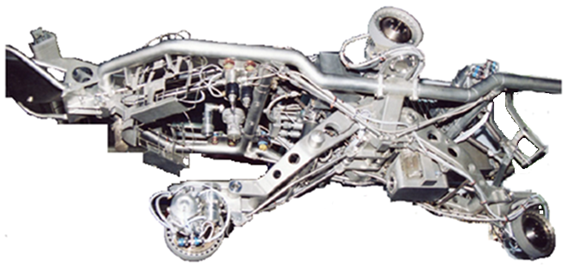
\includegraphics[width=\linewidth]{mir_01}
\end{marginfigure}


\section*{Présentation}
\begin{marginfigure}
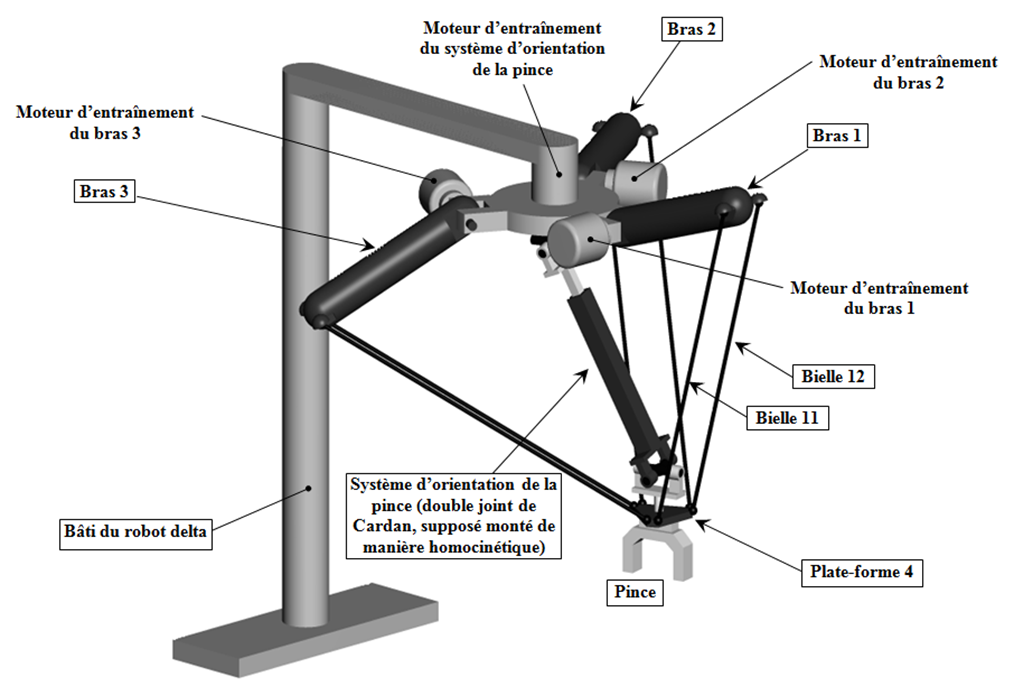
\includegraphics[width=\linewidth]{fig_01}
\end{marginfigure}

Une usine de fabrication de flacons en verre possède un poste de mise en cartons qui est l'objet de la présente étude. Ce poste est équipé de deux robots permettant de déplacer les flacons, déplacer des cartons, détecter des flacons dans des cartons, ranger des flacons dans les cartons.
Ces robots sont de type << Delta >> à architecture parallèle. 


\section*{Architecture de la commande}
On se propose ici de valider le niveau des performances de la commande de l’axe d’orientation de la pince.

\marginnote{Les fonctions dans le domaine temporel seront notées en minuscule, alors que celles dans le domaine de Laplace seront notées en majuscule : par exemple : $\omega(t)$ et $\mathcal{L}(\omega(t))=\Omega(t)$.}

Le servo-entraînement met en rotation un arbre télescopique muni à chacune de ses extrémités d’un joint de Cardan. Le mouvement d’orientation de la pince est indépendant des mouvements de la plate-forme 4. 
Afin d’assurer un bon positionnement angulaire de la pince P, la commande de sa rotation est asservie de la façon suivante :
\begin{itemize}
\item la consigne de position $\theta_{PC}$, entrée par l’utilisateur grâce à une interface graphique (lors des réglages) ou imposée par la Partie Commande (lors des cycles de travail), est transformée en une tension $v_{PC}$ grâce à un convertisseur qui sera assimilé à un système de gain pur $K_C$ (en $\text{V rad}^{-1}$).
\item la vitesse de rotation $\omega_M$ (en $\text{rad s}^{-1}$) et l’angle de rotation $\theta_M$ (en rad) de l’arbre moteur sont mesurés par un codeur incrémental, monté directement sur l’arbre moteur, qui délivre une information numérique; celle-ci est alors transformée par une carte de conversion numérique-analogique (C.A.N.) supposée linéaire en deux tensions $v_{\omega}$ et $v_{\theta}$ telles que :
\begin{itemize}
\item pour la vitesse : $v_{\omega} =K_{\omega}\omega_M$,
\item pour la position : $v_{\theta} =K_{\theta}\theta_M$;
\end{itemize}
\item la tension $v_{\theta}$  (image de la rotation $\theta_M$ du moteur) est soustraite à la tension $v_{PC}$ pour donner la tension $\varepsilon_P$;
\item cette tension $\varepsilon_P$ est modifiée par un correcteur de fonction de transfert $C(p)$ pour donner la tension $\varepsilon_{VP}$;
\item la tension $v_{\omega}$ (image de la vitesse de rotation $\omega_M$ du moteur) est soustraite à la tension $\varepsilon_{VP}$ en sortie du correcteur pour donner la tension $\varepsilon_v$;
\item cette tension $\varepsilon_v$ est amplifiée par un amplificateur de gain pur $G$ pour donner la tension d’alimentation du moteur $u_M$; le moteur tourne alors à la vitesse angulaire $\omega_M$ telle que $\Omega_M(p) = M(p) U_M(p)$;
\item la rotation $\theta_{EC}$ de la pièce d’entrée du double joint de Cardan est telle que $\theta_{EC} = \lambda \theta_M$, grâce au réducteur de vitesse fixé sur l’arbre moteur;
\item le double joint de Cardan est homocinétique et a pour fonction de transfert $R(p) = 1$ (l’entrée est l’angle $\theta_{EC}$, et la sortie est $\theta_{SC}=\theta_P$ où $\theta_P$ est la rotation de la pince fixée sur la pièce de sortie du double joint de Cardan).
\end{itemize}

\question{Tracer le schéma bloc d’asservissement en position, d’entrée $\theta_{PC}(p)$ et de sortie $\theta_{P}(p)$, faisant apparaître toutes les variables et les fonctions de transfert définies ci-dessus.}

\section*{Performances de la commande}
On donne : $\lambda=0,2$ et $K_{\theta}=\SI{0,01}{V.rad^{-1}}$.

\question{On veut que lorsque la pince atteint la position demandée (soit $\theta_P = \theta_{PC}$) l'écart $\varepsilon_P=v_{PC}-v_{\theta}$ soit nul. En déduire la relation entre $K_C$, $K_{\theta}$ et $\lambda$ puis la valeur numérique de $K_C$ qui permette d'assurer cet écart nul.}

\marginnote[-2.5cm]{
Le servo-entraînement utilisé est le AXL305RS330E5 qui est composé du moteur RS330E, du variateur 10/20-60 et du réducteur GB à train épicycloïdal de réduction $\lambda = 0,2$. 
Le moteur RS330E a comme caractéristiques :
\begin{itemize}
\item constante de force électromotrice : $K_E = \SI{14,3}{V/1000 tours.min^{-1}}$;
\item constante de couple : $K_T = \SI{0,137}{N.m.A^{-1}}$;
\item résistance de l’induit : $R_I =\SI{1}{\Omega}$;
\item inductance de l’induit : $L_I = \SI{1,65}{mH}$;
\item frottement visqueux rapporté à l’axe de rotation du moteur négligeable;
\item inertie du rotor + de la charge entraînée rapportée à l’axe de rotation du moteur : $J = 12\times 10^{-5} \text{kg m}^2$.
\end{itemize}}

À partir des équations du moteur à courant continu, on obtient la fonction de transfert suivante : 
$M(p)=\dfrac{\Omega_M(p)}{U_M(p)}=\dfrac{K_T}{K_EK_T +JRp + JLp^2}$. On donne $K_{\omega}=6\,\text{V}/1000 \text{ tours min}^{-1}$.

\question{Déterminer l’expression littérale et la valeur numérique du gain $G$ de l’amplificateur pour que la boucle tachymétrique (d’entrée $\varepsilon_{VP}$ et de sortie $\omega_M$) présente un temps de réponse à 5\% minimum pour une entrée en échelon. Quel est alors le temps de réponse à 5 \% ?}


Avec la valeur de $G$ trouvée précédemment, on a alors calculé la fonction de transfert de boucle (ou en boucle ouverte) suivante pour l’asservissement en position :
$H_B(p)=\dfrac{V_{\theta}(p)}{\varepsilon_P}=C(p)\dfrac{86}{p\left(10^3+3,2 p + 5,3 10^{-3}p^2 \right)}$.


Les exigences de l'orientation du flacon sont données dans le tableau suivant. 
\begin{table*}[!h]
\begin{tabular}{llp{12cm}}
\hline
\textbf{Fonction} & \textbf{Critères} & \textbf{Niveaux} \\ \hline
Orienter le flacon & Stabilité & Marge de phase $M\varphi > 45\degres$  \\
& & Marge de gain $MG>\SI{10}{dB}$\\ 
& Précision & Écart statique nul à une entrée en échelon $\varepsilon_\infty = 0$ \\ 
& Rapidité & Bande passante à \SI{0}{dB} de la fonction $H_B(p)$ : $BP_0 > \SI{50}{rad.s^{-1}}$. On définit la bande passante par sa largeur de bande (ici : \SI{50}{rad.s^{-1}}).
\\ \hline
\end{tabular}
\end{table*}

On considère pour l’instant que le système n’est pas corrigé : $C(p) = 1$.


\begin{marginfigure}
\centering
{\scriptsize
%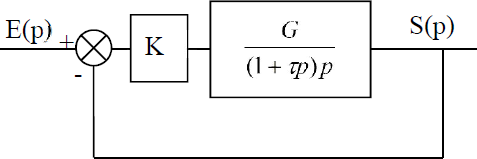
\includegraphics[width=\linewidth]{fig_02}
\begin{tikzpicture}[xscale=1.7,yscale=2]
\AbaqueTRsecond
\end{tikzpicture}}
\end{marginfigure}


\question{Tracer les diagrammes asymptotiques de Bode en amplitude et phase de la fonction de transfert $H_{BO}(p)$ du système non corrigé en plaçant avec précision les points caractéristiques.}

Pour la fin, la courbe de gain sera assimilée à son tracé asymptotique.

\question{Déterminer les valeurs de $M\varphi$, marge de phase, $MG$, marge de gain et $BP_0$, bande passante à \SI{0}{dB} de la fonction de transfert $H_B(p)$. Les critères de la fonction précédente sont-ils vérifiés ?}

\question{Vérifier les valeurs des marges par le calcul.}


On prend une correction proportionnelle : $C(p) = C_0$.
\question{Déterminer la bande de valeurs de $C_0$ qui permettent de vérifier les critères du cahier des charges partiel donné précédemment.}


\ifprof
\else
\begin{marginfigure}%[-5cm]
\centering

\includegraphics[width=3cm]{Cy_02_Ch_01_Colle_06_Prehenseur_qr}
\end{marginfigure}
\fi

